\documentclass{ctexart}
\usepackage{enumerate}
\usepackage{graphicx}
\newcommand{\tmaffiliation}[1]{\\ #1}

\begin{document}
\title{路由器组实验报告}

\author{
  陈嘉杰
  \tmaffiliation{计72班\\
  2017011484}
  \and
  赵博文
  \tmaffiliation{计72\\
  2017011410}
}
\date{2019年6月30日}
\maketitle
\tableofcontents

\section{项目概况}
\subsection{项目目标}
  路由器项目的目标是,在FPGA上实现一个四口路由器,实现硬件的三层转发功能,并且把数据平面的工作转交CPU上的软件实现,允许软件动态更新转发表并且读取统计数据。

  除了转发功能,硬件部分还应该实现以下的目标:

  \begin{enumerate}
    \item 四个端口全双工
    \item 保证以完整的以太网帧单位进行丢包
    \item 保证各端口之间流量的公平性
  \end{enumerate}

  除了硬件以外,软件部分还需要重新实现网络原理课程的实验内容,即实现一个支持 RIP 协议的路由,它从硬件部分读取部分需要处理的以太网帧,并实现 RIP 协议与链路上的其它 RIP 路由器进行路由信息的交换。它应该实现这些功能:

  \begin{enumerate}
    \item 正确响应 ARP 请求
    \item 定时广播自己的 RIP 路由表信息
    \item 接收并解析 RIP 信息,更新路由表
    \item 定时对路由表表项进行更新,并写入到硬件的转发表
  \end{enumerate}

  为了展示效果,额外添加了 HDMI 的输出,使得用户可以直观地看到当前的路由表信息和各个端口进出的流量。

\subsection{项目结构}
  为了支持更多平台和将来的使用,项目的结构比较复杂,主要分为以下几个子项目:

  \begin{description}
    \item[naiverouter] 封装成 IP 的路由转发核心,提供和CPU交换数据的通道和四个 RGMII 接口。
    \item[router]  在 AX7021 平台上,软件运行在 ARM 处理器上的完整路由器实现,在 Xilinx SDK 中采用 C 语言实现了 RIP 协议和 HDMI 的可视化输出。
    \item[router\_mb] 也是在 AX7021 平台上,软件则是运行在 FPGA 中的 MicroBlaze  核,在 Xilinx SDK 中实现了与路由器的交互逻辑,实现了 ARP 的响应和转发表的读取。
    \item[router\_ksz8795] 在 Pynq-Z1 开发板外接一个带有 KSZ8795 和四个网口的扩展板平台上,软件运行在 FPGA 中的 MicroBlaze 核,采用软路由的方式进行转发,底层采用的是新设计的统一接口的 HAL 库。
  \end{description}

  其中 router 项目为最早出现的子项目,首先作为一个纯硬件项目开始开发,实现完硬件转发后,开始实现软件部分,继续扩展后,为了测试在不同平台和情况下的使用,把它分离出单独的 naiverouter 项目,以一个独立的 IP 的形式加入到其余的项目之中。

\section{具体实现}
\subsection{硬件部分(NaiveRouter)}
\subsubsection{总体架构}
  考虑到需要保证四个端口同时互相转发的流量,在设计的时候选择了如下的方案:
  
  \begin{itemize}
    \item 设计一个 4*4 (后来加上到 CPU 之后实际上是 5*5) 的转发通路,每一个端口都可以向每一个端口发送以太网帧(包括自己),每个端口通过轮询的方式选择从哪个端口接收数据,保证公平性。
    \item 设计了一个全局的 ARP 表,通过仲裁的方式保证端口之间操作的原子性。考虑到操作 ARP 表使用的周期相比数据并不多,所以并没有为每个端口设置一个 ARP 表。即使是每个端口一个 ARP 表,也不能解决转发目标是同一个端口时,需要同时查询同一个 ARP 表的问题,但可以减少仲裁的等待时间。
    \item 设计了一个全局的转发表,和 ARP 表类似。出于同样的考虑,没有在每个端口设置一个转发表,但设置多个转发表确实可以免去仲裁的一步,只是在软件更新转发表的时候需要更多一步操作。
  \end{itemize}

\subsubsection{转发矩阵}
  转发矩阵是一组 4*4 (5*5)交叉连接的接口,每个接口包含这些端口:

  \begin{description}
    \item[wdata] 逐字节的数据
    \item[wlast] 表示一个以太网帧最后一个字节
    \item[wvalid] 表示发送端可以发送数据
    \item[wready] 表示接收端可以接收数据 
  \end{description}

  只有当 wvalid 和 wready 同时为高时,才会传输数据,与 AXI-Stream 类似。但与 AXI-Stream 不同的是,为了简化逻辑,这里的 wvalid wready wdata 并不在同一个周期上升,而是等待一个周期后开始正式传输。

  对于连接到物理网口的端口来说,并不需要区分它来自哪里,但是软件部分需要按照这个来做一些处理,也需要特定的方法告诉硬件部分应该从哪个端口出。因此,额外添加了一段逻辑,在以太网帧最前面加上一个数字,代表端口号,这样就可以区分是从哪个端口入,需要从哪个端口出。

\subsubsection{ARP 表}
  前面已经提到过,为什么采用了全局的 ARP 表而没有选择每个端口单独一个 ARP 表。它的实现也很简单,就是在 BRAM 中保存一个简单的哈希表,简单按照 IP 地址选择后,就按顺序在桶内部顺序查找。更新也是类似,找到对应的桶后,如果找不到对应的 ARP 表项,就把新的 ARP 表项插入到最前面。由于不需要支持太多设备,所以这个表并不是很大。

  它提供了简单的接口,一个是查询,一个更新。采用了类似的 valid 和 ready 信号,最后输出查询的结果和插入的完成信息。在外层套一个仲裁,就变成了实际使用的 ARP 表。

  在写入 ARP 表的时机选择上,采取了接受到一个 ARP 请求/回复的时候,按照 Sender IP 和 Sender MAC Address 来插入。这样免去了在大量 IP 转发时不断更新 ARP 表,也能保证正确性和效率。

  在 router/docs/ 下有一个单独的 ARP 表的文档。

\subsubsection{转发表}
  转发表和 ARP 表类似,也是一个数据结构,但是为了保证最长匹配,要求转发表中的表项按照前缀长度不降来排列,这样只要找到第一条匹配的,就可以保证是最长匹配。有一些论文探讨了如何采用更高效的树的接口来进行同样的操作,在本次实验中并没有实验,留作后人继续改进。

  它提供了简单的接口,一个是查询,一个是 BRAM 的接口,用于转发表的更新。查询也采用了类似的 valid 和 ready 信号,最后输出查询的结果。也在外层加了一个仲裁,然后给各个端口使用。

  在实现了软件动态更新转发表之前,通过初始化的数据实现了一个静态的转发表。通过把 BRAM 的接口暴露出去,接到 AXI BRAM Controller 后,就可以很方便地实现转发表的动态更新。

\subsubsection{核心转发逻辑}
  这是最复杂的部分,包含两个方向的数据通路,和多个部分进行互操作,在每一个端口下都有同样的一份逻辑。它有两种工作模式:一个是纯硬件,在硬件中处理 ARP 的回应和 ARP 表查询不到时发出对应的请求;一个是软硬结合,把符合一定条件的以太网帧都发送给CPU交由软件处理,剩下就按照转发表进行处理。

  首先是从物理网口开始,到转发引擎,修改后再转发出去的数据通路,也是比较复杂的一段。主要分以下几个流水线步骤:

  \begin{enumerate}
    \item 从 MAC 过来的数据要求接受者随时可以接收,所以添加了一个 FIFO 进行缓存。但是现成的 FIFO 并不支持以完整的以太网帧的单位进行舍弃,于是拆分成了两个FIFO,一个存数据,一个存长度,先写入数据后写入长度,保证原子性。在剩余空间不足一个完整的以太网帧的时候,直接丢弃。
    \item 从上一步读取一个以太网帧,先读长度后读数据,和上面匹配。在读取的同时,进行一系列的解析和处理:拆分出需要特殊处理的一些数据,如接受者 MAC,发送者 MAC,EtherType,ARP 和 IP 的信息。
    \item 如果是 ARP ,提取出它的 Sender IP 和 Sender MAC ,保存到 ARP 表中。如果是纯硬件转发模式,如果 Target IP 匹配到自己的地址,需要构造一个回应。否则就选择转发给 CPU 。
    \item 如果是 IP ,判断目的地址,如果是广播和组播地址,就转发给 CPU ;否则,查询转发表,得到下一跳的 IP 地址和出端口信息,接着查询下一跳的 MAC 地址,得到新的目的 MAC 地址和 IP 头中 TTL 和 Checksum 。
    \item 如果前两步得到了需要发送的结果,向指定的端口发送以太网帧,即拉高 valid ,等待对方 ready 后开始传输,传输到最后一个字节 last 拉高,valid 拉低,完成一次完整的转发操作。
  \end{enumerate}

  以上的步骤,都是流水线操作,等到前一步得到足够的信息后立即开始下一步,如转发 IP 包时,只要读取到 IP 头中的目的 IP 地址信息就开始查询,这样可以保证转发的效率,这就是为什么把 ARP 表和转发表放全局并不会带来太多的性能损失的原因。

\subsection{软件部分(ARM/MicroBlaze over AX7021/Pynq)}
  在实现完硬件部分后,就开始了软件部分的编写。最初的目标就是实现一个 RIP 路由器,后来在这个基础上又增加了 HDMI 的可视化输出功能,最后移植一部分功能到 MicroBlaze 和 Pynq-Z1 with KSZ8795 平台上。

  最初实现一个可用的 ARM 上运行的软硬结合的路由器大概需要这些步骤:

  \begin{itemize}
    \item 修改硬件部分,使得它可以给 CPU 收/发以太网帧,也可以让 CPU 读写转发表,并读取统计信息,具体的实现方法在上面硬件部分已经有讲述。
    \item 在 Xilinx SDK 中采用 Xilinx 提供的 BSP 里对应的驱动:AXI Bram Controller,AXI-Stream FIFO 和 AXI GPIO 来和硬件部分交互,分别负责转发表的更新,以太网帧的收发和统计数据的读取。
    \item 接着,用 C 代码实现简单的轮询,不断从 AXI-Stream FIFO 中读取以太网帧,并注册一个时钟中断,每秒进行一次更新,输出当前状态并把路由表写入转发表。
    \item 接着实现 ARP 响应,RIP的接收和广播,按照规则更新路由表。
    \item 最后添加 HDMI 输出,通过 VDMA 把 FrameBuffer 更新到视频输出,以 20fps 的帧率更新显示,手动绘制各个图案和文字。
  \end{itemize}

  \begin{figure}[htbp]
    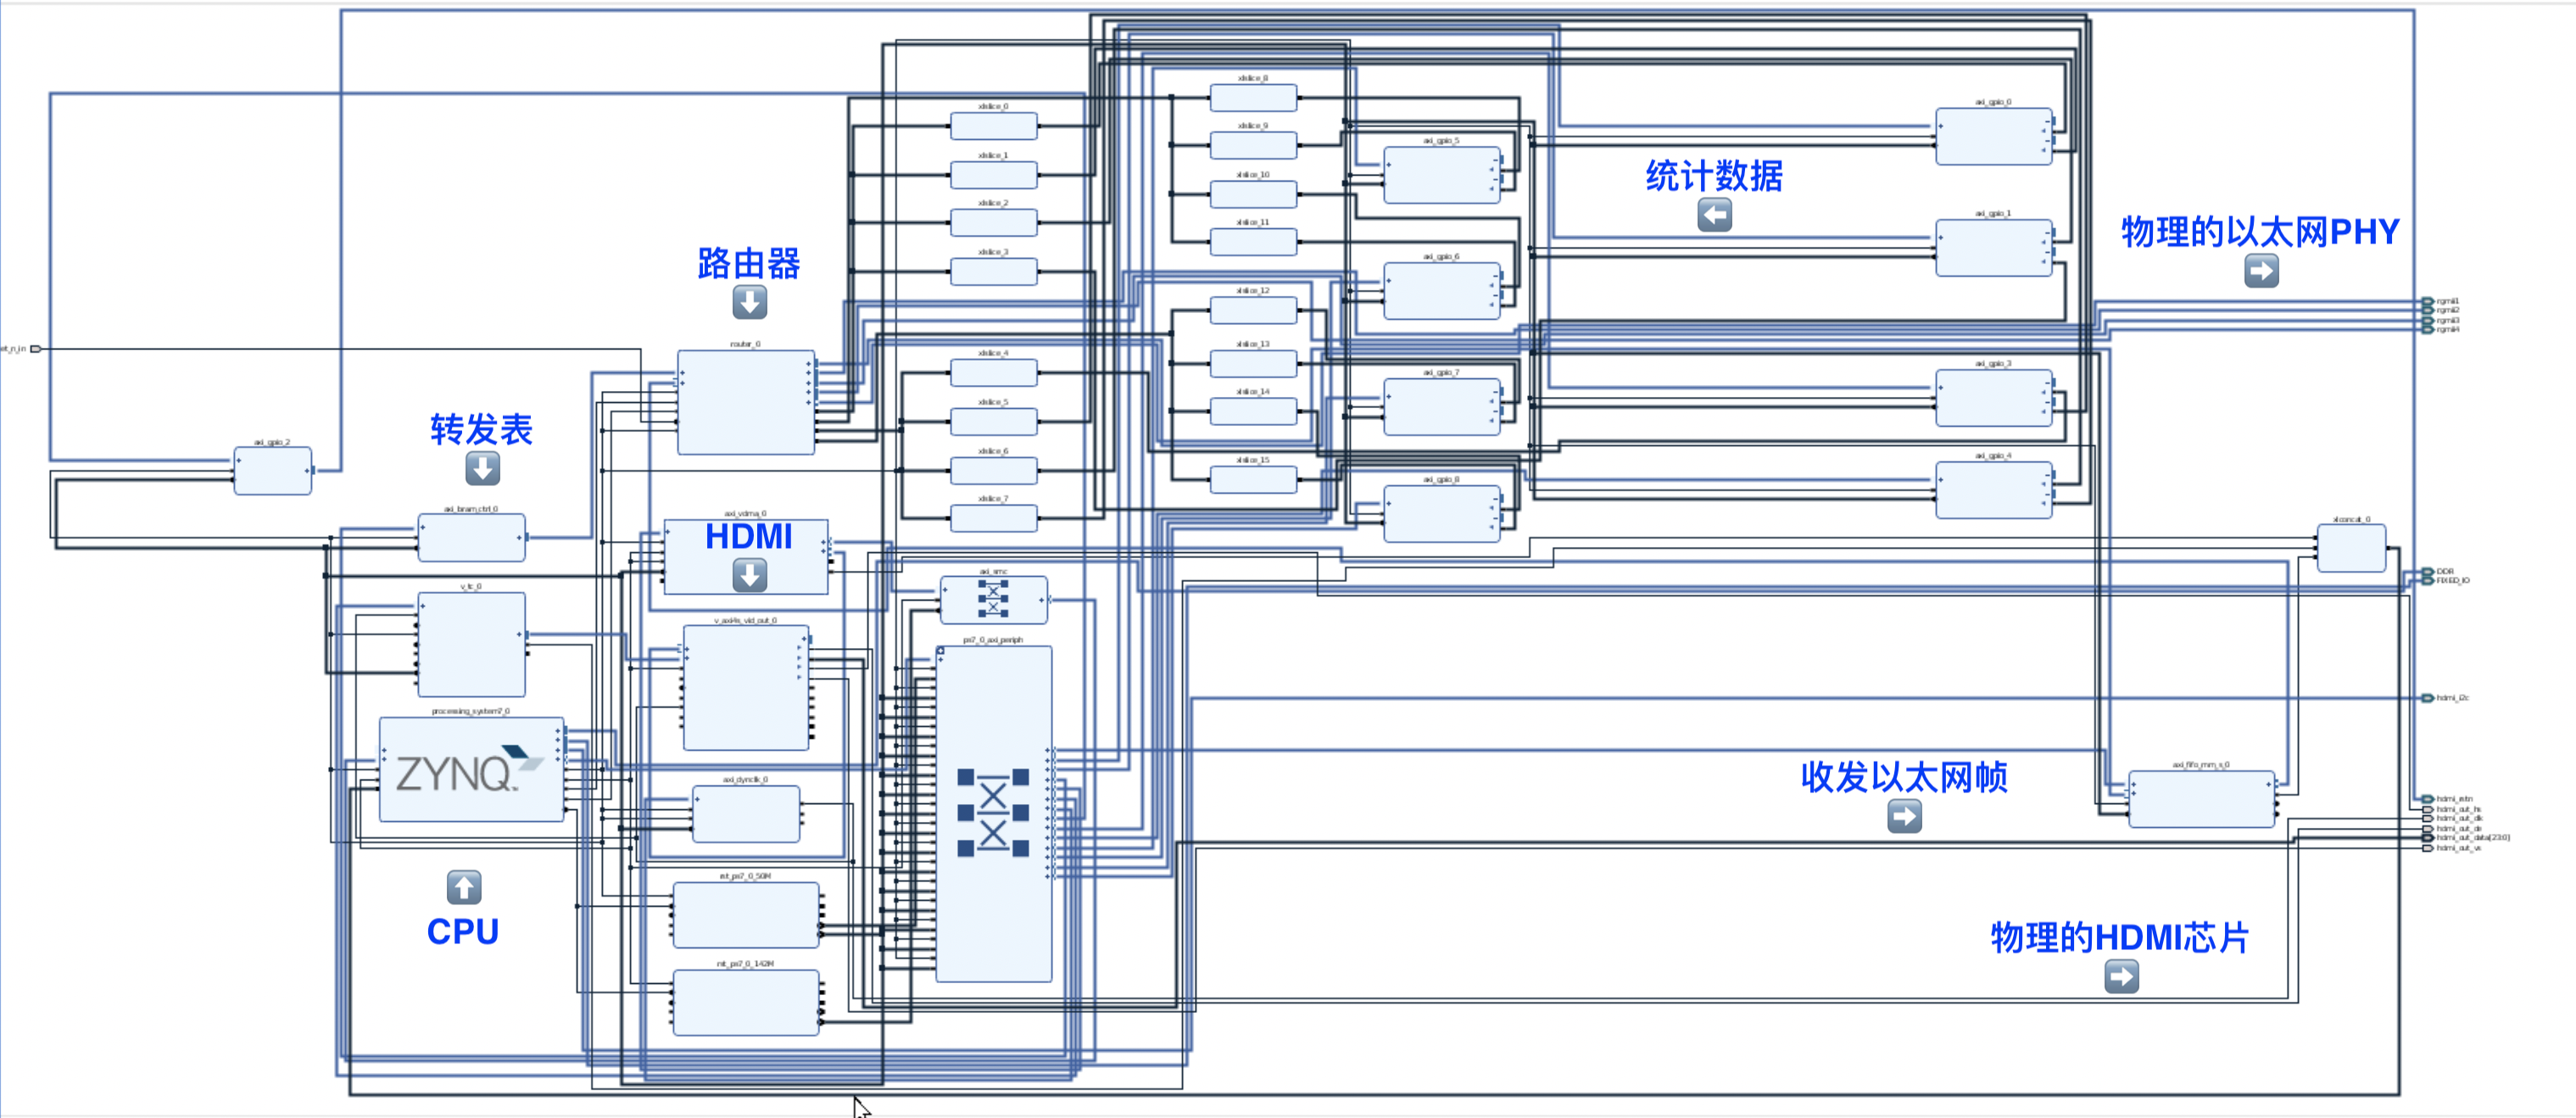
\includegraphics[width=\linewidth]{router.png}
    \caption{组件之间连接的图示}
  \end{figure}
\end{document}
